\documentclass{beamer}
\usetheme{Boadilla}

\usepackage{statmath}
\usepackage{amsmath}
\usepackage{subcaption}
\usepackage{amsfonts}
\usepackage{graphicx}
\usepackage[demo]{graphicx}
\usepackage{subfig}
\usepackage{caption}
\usepackage{tabularx}


\usepackage{tablefootnote}
\usepackage{amssymb}
\usepackage{float}
\usepackage[colorinlistoftodos]{todonotes}
\usepackage{geometry}
\usepackage{booktabs}
\usepackage{siunitx}
\usepackage{tabularx}
\usepackage{placeins}
\usepackage{booktabs}
\usepackage{xcolor}
\usepackage{colortbl}
\usepackage{multirow}
\usepackage[acronym]{glossaries}
\usepackage{indentfirst}
\usepackage{algorithm}
\usepackage{algorithmic}





\usepackage[
  backend=biber,
  style=alphabetic,
  maxbibnames=10,
  minalphanames=2,
  citestyle=authoryear-comp, 
  sorting=nyt
]{biblatex}
\addbibresource{biblio.bib}
\usepackage[colorlinks=true,linkcolor=blue,citecolor=blue,urlcolor=blue]{hyperref}
\hypersetup{
    colorlinks=true,
    linkcolor=blue,
    citecolor=blue,
    urlcolor=blue
}



\setbeamertemplate{caption}[numbered]
\title{Prédiction des parcours ratés}
\author{JAYLET Olivier}


\begin{document}
\begin{frame}
  \titlepage
\end{frame}

\begin{frame}{Outline}
    \begin{itemize}
        \item Introduction
        \item State of the art
        \item Dataset \& Descriptive Statistics
        \item Noise generation on path duration
        \item Selected Machine Learning Models
            \begin{itemize}
                \item Classification models
                \item Probability calibration models
            \end{itemize}
        \item Methodology
            \begin{itemize}
                %\item Data normalization
                \item Data splitting
                \item Cross validation
                \item Hyper-parameter optimization
                \item Overview
            \end{itemize}
        \item Classification analysis
            %\begin{itemize}
            %    \item Predicted score analysis
            %    \item Searching for the best classification threshold
            %    \item Classification performance
            %\end{itemize}
        \item Probability calibration analysis
        \item Conclusion
    \end{itemize}
\end{frame}
    
\begin{frame}{Introduction} 
    
    \begin{itemize}
        \item ADP objectives : 
            \begin{itemize}
                \item Ensure the best possible passenger services.
                    \begin{itemize}
                        \item Ensure safety.
                        \item Manage and respect flight schedules.
                        \item Make airport journeys smooth and pleasant.
                        \item \textbf{Do not lose my baggage !!!}
                    \end{itemize}
            \end{itemize}

    \item Lever available to reduce mishandled bags : 
        \begin{itemize}
            \item New infrastructure construction.
            \item Review of current logistics processes.
            \item Cause of mishandled baggage analysis.
            \item \textbf{Prediction of mishandled baggage} in order to : 
                \begin{itemize}
                    \item Remove baggage to avoid unnecessary bottleneck of infrastructures.
                    \item Create a new logistics process for baggage with a high probability of being mishandled (if processed by BHS).
                \end{itemize}
        \end{itemize}

    \end{itemize}
    
\end{frame}

    
\begin{frame}{Introduction} 
    \begin{itemize}
        \item What does my study provide ? 
            \begin{itemize}
                \item A classification model of mishandled baggage (binary prediction)
                \item An accurate probability of being mishandled
            \end{itemize}
        \item When should my model run ? 
            \begin{itemize}
                \item At the baggage entrance to the BHS
            \end{itemize}
    \end{itemize}    
\end{frame}



\begin{frame}{State of the art} 

Several studies on the logistic were found, but only one was aimed at forecasting mishandled baggage.\hfill \break

\cite{MishandledBgas} trained and tested a Light Gradient Boosting model to predict for each bag a probability of being a mishandled baggage. The aim of this study is to identify "at-risk" baggage. \hfill \break
\begin{itemize}
    \item Trained a logistic regression as a benchmark model
    \item None of the data used comes from the BHS, but only from data known by an airline.
    \item Oversampling was used to overcome the unbalanced dataset issue.
    \item The best model has a recall of 0.565, a precision score of 0.506 and an F1 score of 0.534.
\end{itemize}
\end{frame}



\begin{frame}{Dataset}

\begin{figure}
        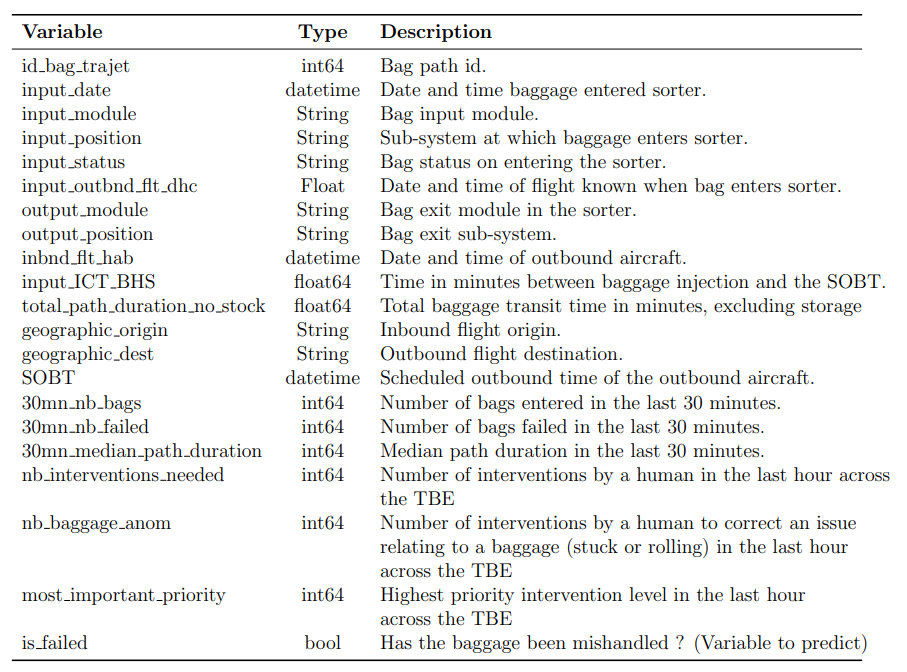
\includegraphics[width=0.7\linewidth]{data table.png}
        \caption{Dictionary of Variables}
\end{figure}

\centering
Date : 1st August 2023 - 31st October 2023

\end{frame}






\begin{frame}{Descriptive statistics} 
\begin{figure}[ht]
  \centering
  \begin{subfigure}{0.45\textwidth}
    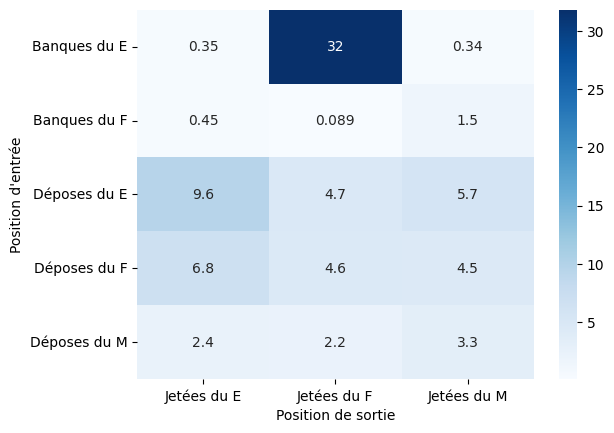
\includegraphics[width=\linewidth]{percentage of failed per positions.png}
    \caption{Percentage of mishandled bags according to input and output positions}
    \label{fig:Percentage of mishandled bags according to input and output positions}
  \end{subfigure}
  \hfill
  \begin{subfigure}{0.48\textwidth}
    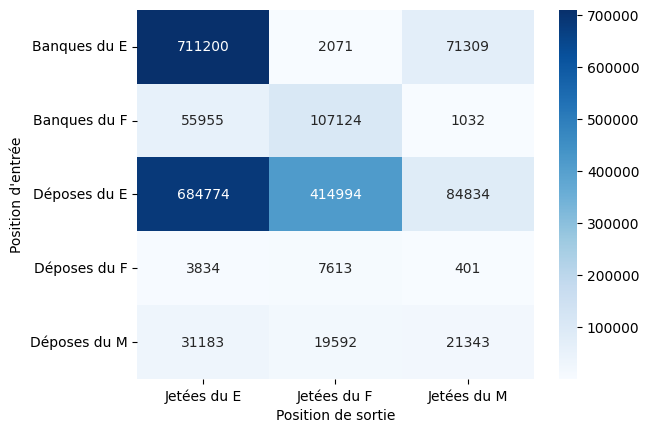
\includegraphics[width=\linewidth]{number of bags per positions.png}
    \caption{Number of bags according to input and output positions}
    \label{fig:Number of bags according to input and output positions}
  \end{subfigure}
  \caption{Mishandled bags according to positions}
  \label{fig:Mishandled bags according to positions}
\end{figure}
\end{frame}



\begin{frame}{Descriptive statistics} 
    \begin{figure}[h]
        \centering
        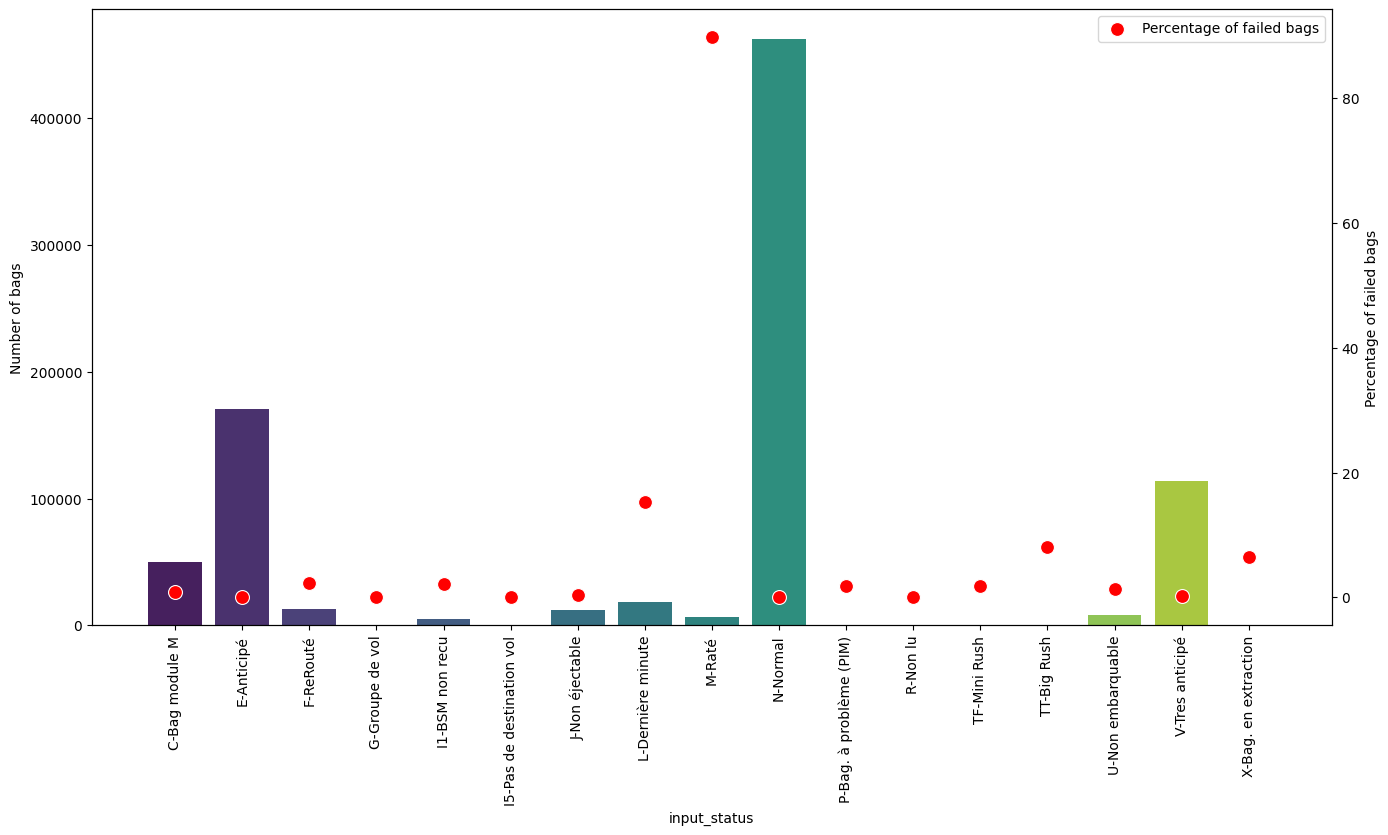
\includegraphics[width=0.9\textwidth]{failed bags per input status.png}\\
        \caption{Number and percentage of failed bags per input status}
        \label{fig:Number and percentage of failed bags per input status}
    \end{figure}
\end{frame}



\begin{frame}{Path duration impact}
    \begin{figure}[h]
        \centering
        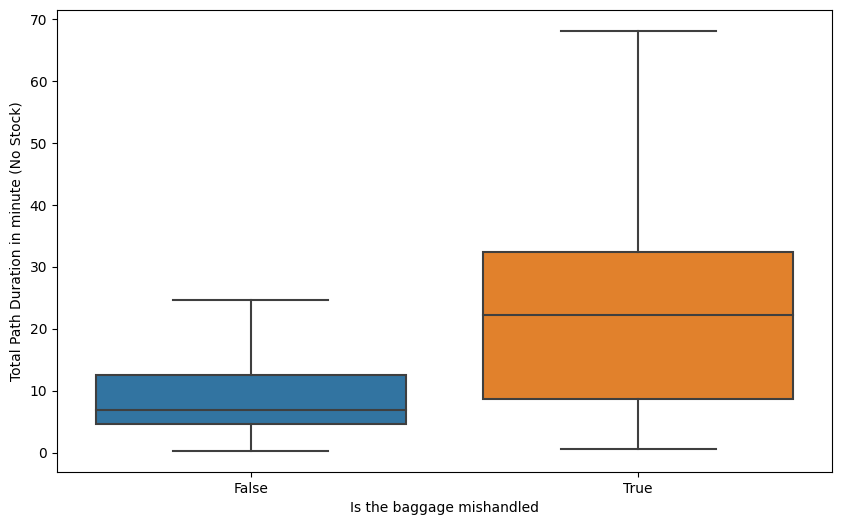
\includegraphics[width=0.6\textwidth]{Boxplot path duration per failed status.png}\\
        \caption{Distribution of paths duration for successed and mishandled bags (without outliers)}
        \label{fig:Distribution of paths duration for non-failed and failed bags}
    \end{figure}
\end{frame}





\begin{frame}{Noise generation on path duration}

\begin{itemize}
    \item Path duration is known once the path exits the BHS.
    \item Thus, using this data makes no sense.
    \item But path duration can be predicted beforehand (see Miracle's study\footnote{Merci Monsieur Miracle}).
    \item In the future : we could use predicted path duration as a proxy. 
    \item In my study : I generate noise according to path duration prediction residuals, and add them to the actual path duration.
\end{itemize}


\begin{table}[h]
  \centering
  \caption{Path duration quantiles}
  \label{tab:Path duration quantiles}
  \begin{tabular}{|c|c|c|}
        \toprule
        \textbf{Quantiles} & \textbf{Path Duration (in minute)}  \\
        \midrule
        Q1 & 4.4  \\
        Q3 & 17  \\
        D9 & 28.4  \\
        P99 & 53.3  \\
        \bottomrule
  \end{tabular}
\end{table}
\end{frame}


\begin{frame}{Noise generation on path duration} 

\begin{figure}[ht]
  \centering
    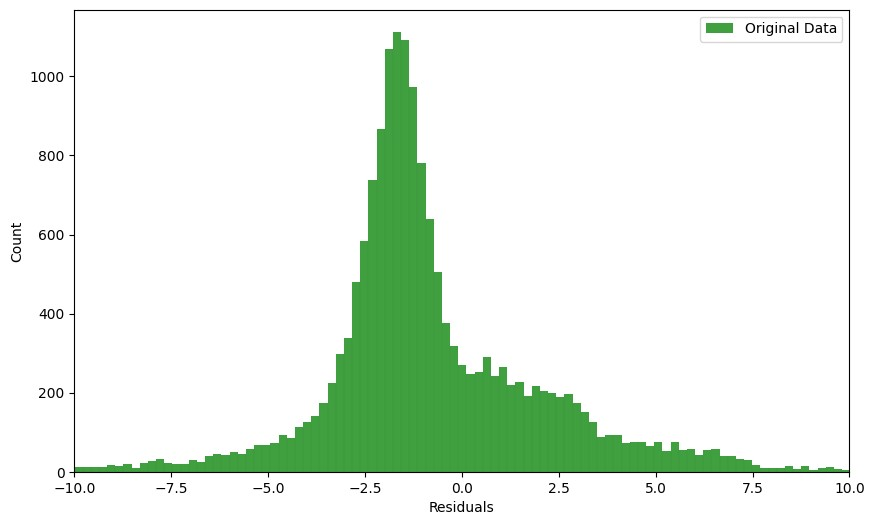
\includegraphics[width=\linewidth]{Q1_Q3 distribution.jpg}
    \caption{Distribution of residuals (Q1 $<$ Path duration $<$ Q3)}
    \label{fig:Distribution of residuals for path duration between Q1 and Q3}
\end{figure}
\end{frame}

\begin{frame}{Noise generation on path duration} 
\begin{figure}[ht]
  \centering
    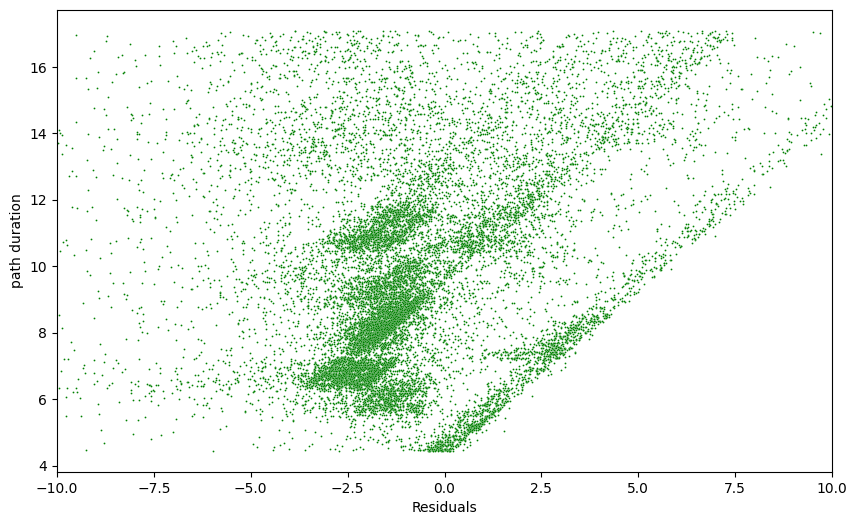
\includegraphics[width=\linewidth]{Q1_Q3 residuals path duration.png}
    \caption{Scatter plot of residuals Vs. path duration (Q1 $<$ Path duration $<$ Q3)}
    \label{fig:Scatter plot of residuals Vs. path duration (Q1 < time duration < Q3)}
\end{figure}
\end{frame}



\begin{frame}{Noise generation on path duration} 
    \begin{itemize}
        \item Generation methodology :
        \begin{itemize}
            \item Estimate a kernel density estimation of residuals.
            %\begin{equation}
            %f(x) = \frac{1}{nh} \sum_{i=1}^{n} K\left(\frac{x - x_i}{h}\right)
            %\end{equation}
    
            \item Generate a new dataset from this density estimation.
            \begin{itemize}
                \item Output : generated path duration and residuals.
            \end{itemize}
            \item For each actual path duration : 
            \begin{itemize}
                \item Find the nearest generated path duration (with a binary search algorithm).
                \item Assigns a residual to each actual path duration.
                \item Add up actual path duration and assigned generated residual.
                \item If  path duration + residual $<$ 0 : add up the residual absolute value.
    
            \end{itemize}
        \end{itemize}
    \end{itemize}
\end{frame}






\begin{frame}{Noise generation on path duration} 
\begin{figure}[ht]
  \centering
    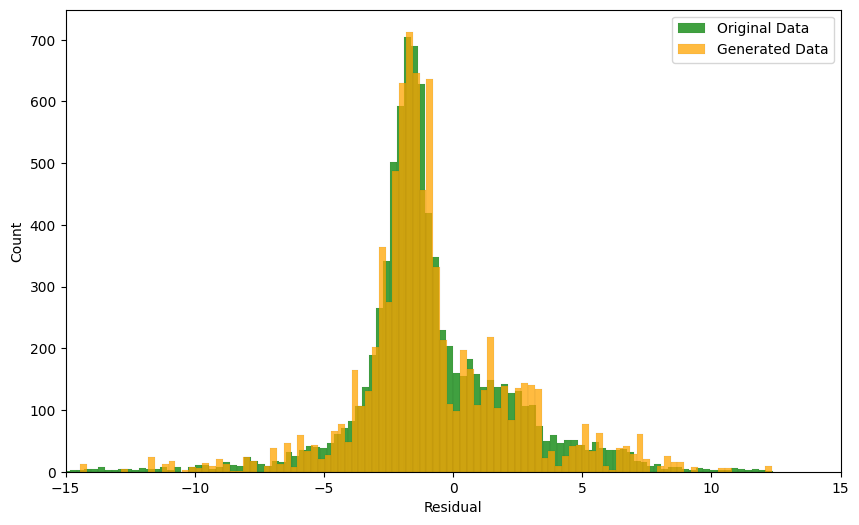
\includegraphics[width=\linewidth]{Q1_Q3 distribution actual Vs. generated.png}
    \caption{Distribution of actual Vs. generated residuals (Q1 $<$ TMP $<$ Q3)}
    \label{fig:Q1_Q3 distribution actual Vs. generated}
\end{figure}
\end{frame}

\begin{frame}{Noise generation on path duration} 

\begin{figure}[ht]
    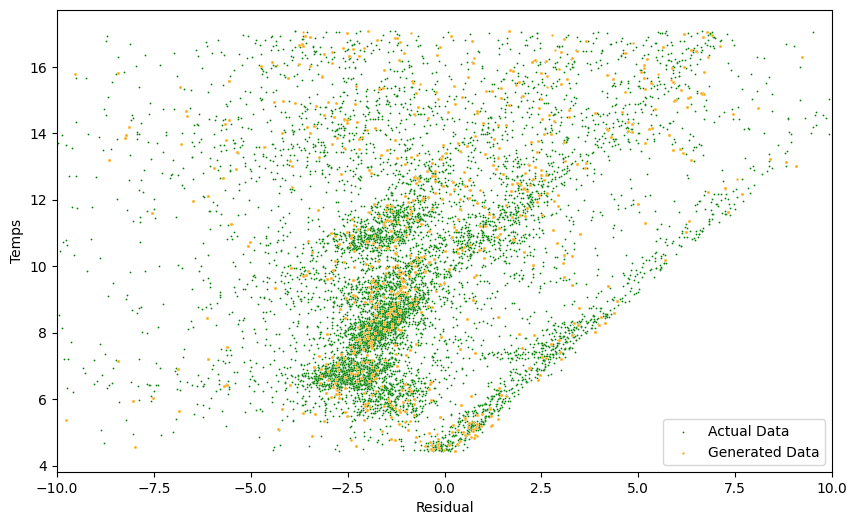
\includegraphics[width=\linewidth]{Q1_Q3 actual Vs. generated.png}\\
    \caption{Actual Vs. generated residuals}
    \label{fig:Actual Vs. generated residuals (Q1 < time duration < Q3)}
\end{figure}

\end{frame}



\begin{frame}{Noise generation on path duration}

\begin{figure}[h]
    \centering
    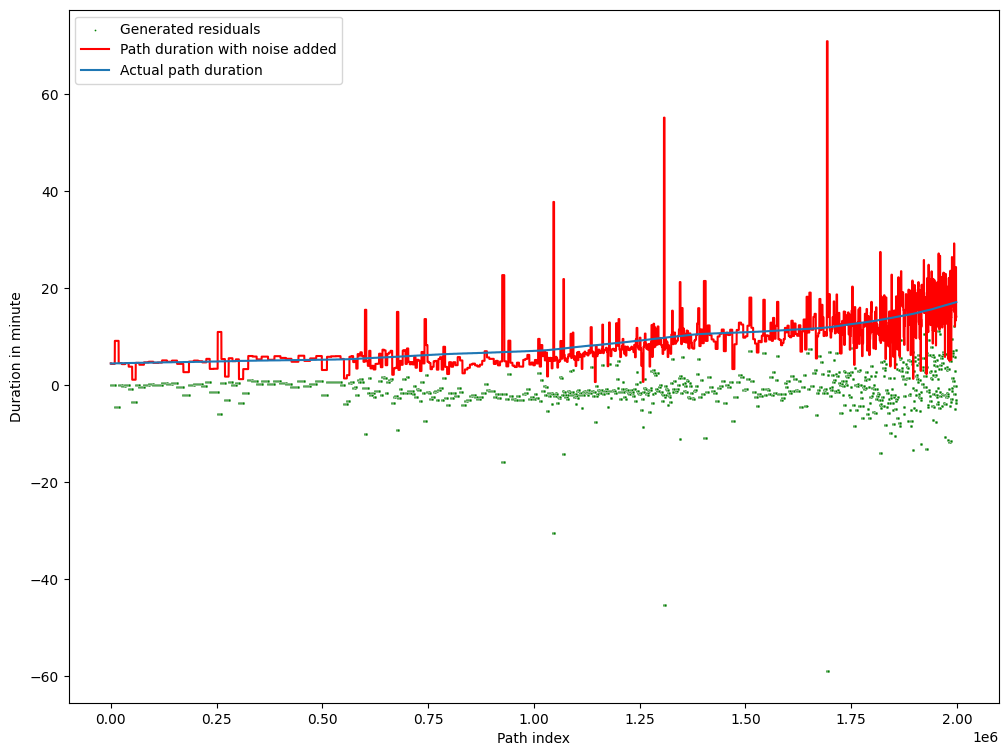
\includegraphics[width=0.8\textwidth]{Q1_Q3 path duration noised.png}\\
    \caption{Comparison of actual path duration with path duration with noise added (Q1 $<$ Path duration $<$ Q3)}
    \label{fig:Q1_Q3 path duration noised.png}
\end{figure}
    
\end{frame}

\begin{frame}{Selected Machine learning models}

\begin{itemize}
    \item Classification models
    \begin{itemize}
        \item Logistic regression as a benchmark model
        \item Random Forest
        \item Extreme gradient boosting
    \end{itemize}
    \item Probability calibration models
    \begin{itemize}
        \item Platt scaling
        \item Isotonic regression
    \end{itemize}
\end{itemize}
    
\end{frame}


\begin{frame}{Probability calibration}

Why should we calibrate probabilities ?
\begin{itemize}
    \item A classification model classifies data according to a predicted score (between 0 and 1).
    \item This score cannot be interpreted as a probability.
    \item Calibration models transform  predicted scores into actual probabilities.
    \begin{itemize}
        \item Platt scaling is a logistic regression and isotonic regression a non-parametric estimation. 
        \item Both take the predicted scores as input and the true label as target.
    \end{itemize}
\end{itemize}

    
\end{frame}


\begin{frame}{Methodology}
\begin{figure}[h]
    \centering
    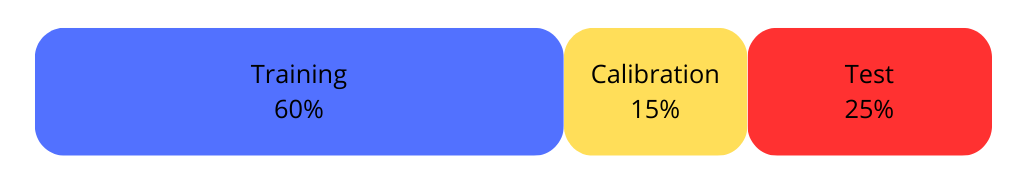
\includegraphics[width=0.7\textwidth]{Data splitting.png}\\
    \caption{Data split}
    \label{fig:Data split}
\end{figure}
\begin{figure}[h]
    \centering
    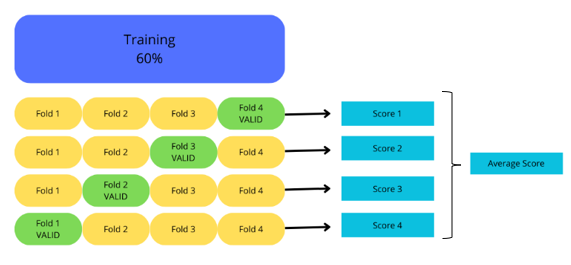
\includegraphics[width=0.65\textwidth]{KFold data.png}\\
    \caption{Stratified KFold cross-validation}
    \label{fig:KFold cross-validation}
\end{figure}
\end{frame}


\begin{frame}{Hyper-parameter optimization}
\begin{figure}[h]
    \centering
    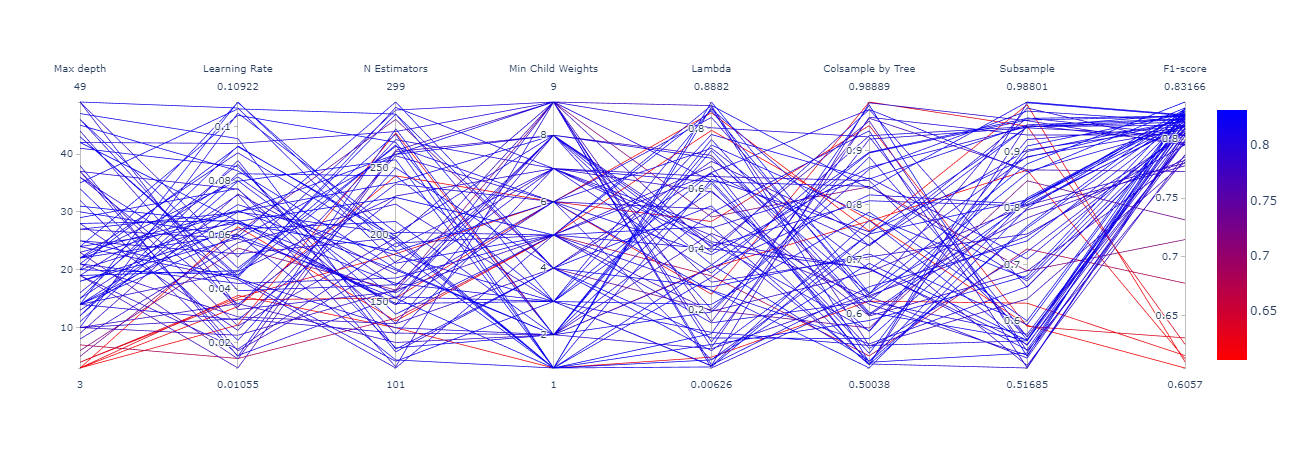
\includegraphics[width=1\textwidth]{Random search XGB.png}\\
    \caption{Parallel coordinate plots for hyper-parameter optimization}
    \label{fig:Random search XGB}
\end{figure}
\end{frame}


\begin{frame}{Hyper-parameter optimization}
\begin{figure}[h]
    \centering
    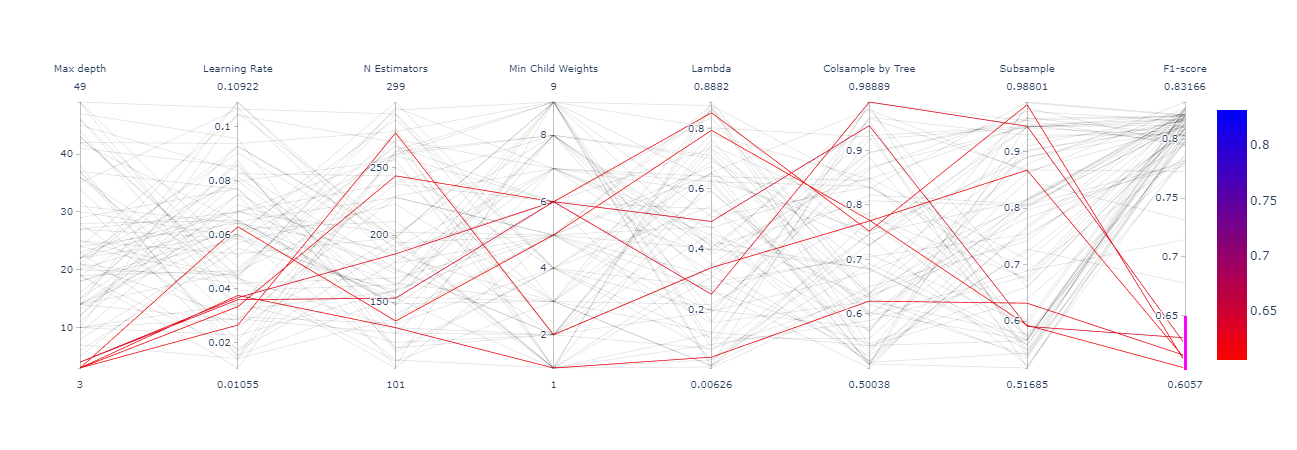
\includegraphics[width=0.75\textwidth]{Random search XGB 2.png}\\
    \caption{Focus on inefficient parameters}
    \label{fig:Random search XGB 2}
\end{figure}
\begin{figure}[h]
    \centering
    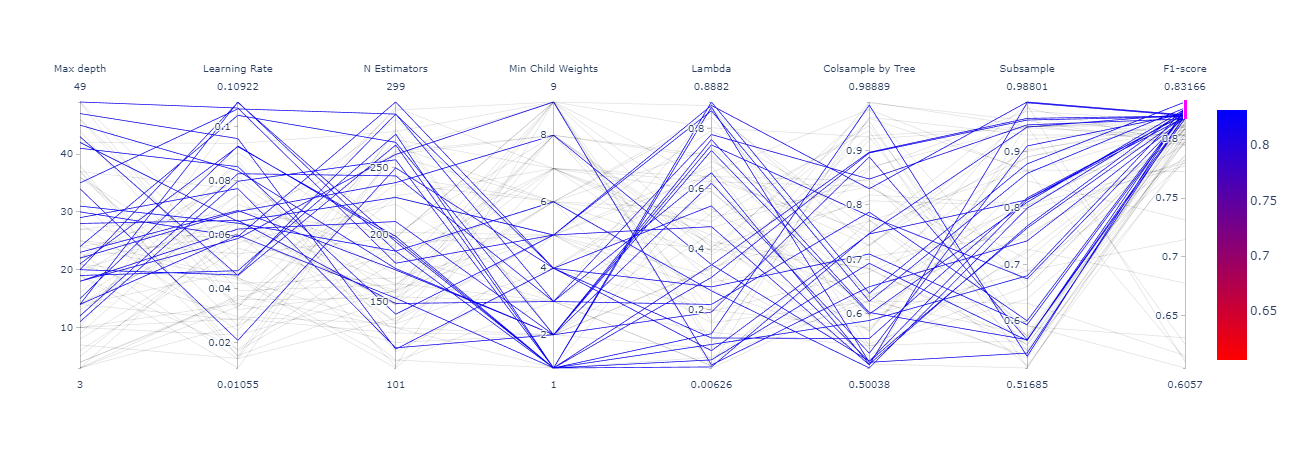
\includegraphics[width=0.75\textwidth]{Random search XGB 3.png}\\
    \caption{Focus on efficient parameters}
    \label{fig:Random search XGB 3}
\end{figure}
\end{frame}

\begin{frame}{Methodology overview}
\begin{figure}[h]
    \centering
    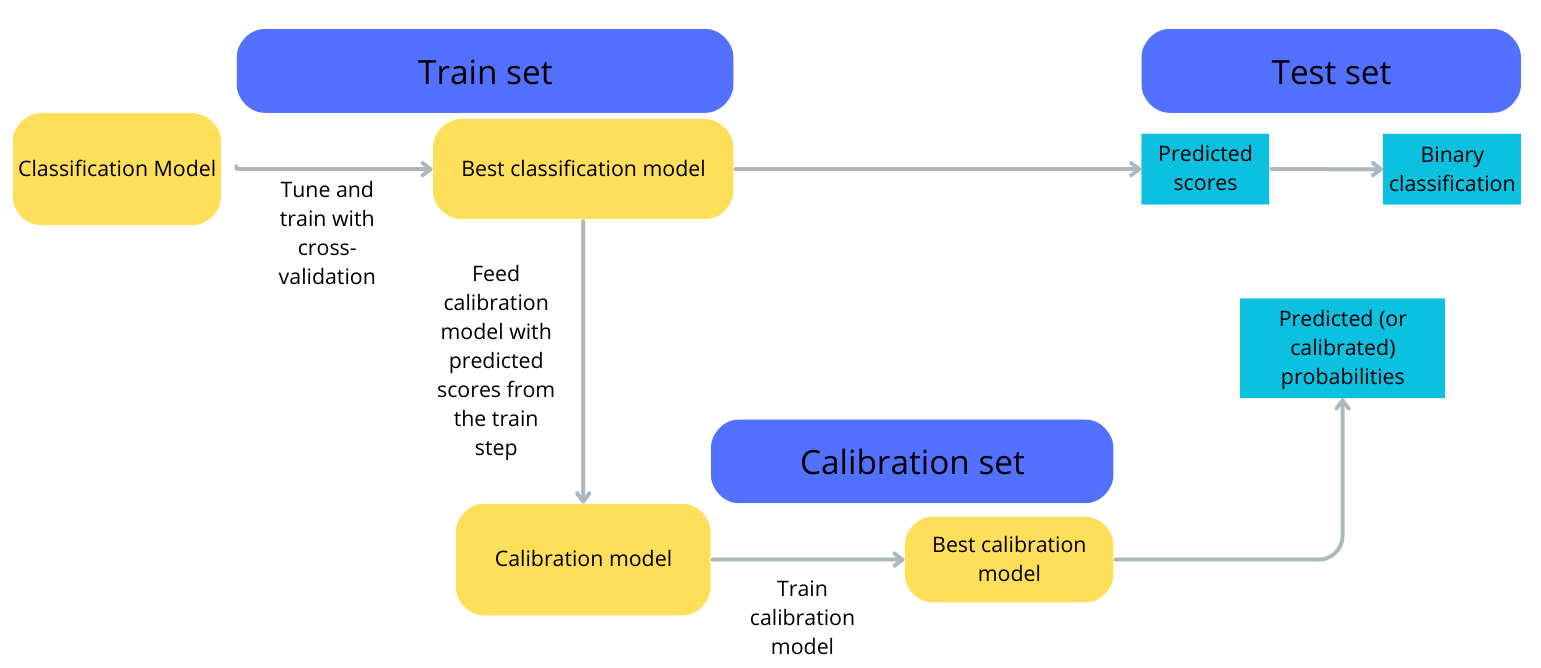
\includegraphics[width=1\textwidth]{Methodology.png}\\
    \caption{Training, calibration and testing methodology}
    \label{fig:Methodogoly}
\end{figure}
\end{frame}



\begin{frame}{Classification analysis} 
\begin{figure}
\begin{minipage}[c]{0.4\linewidth}
    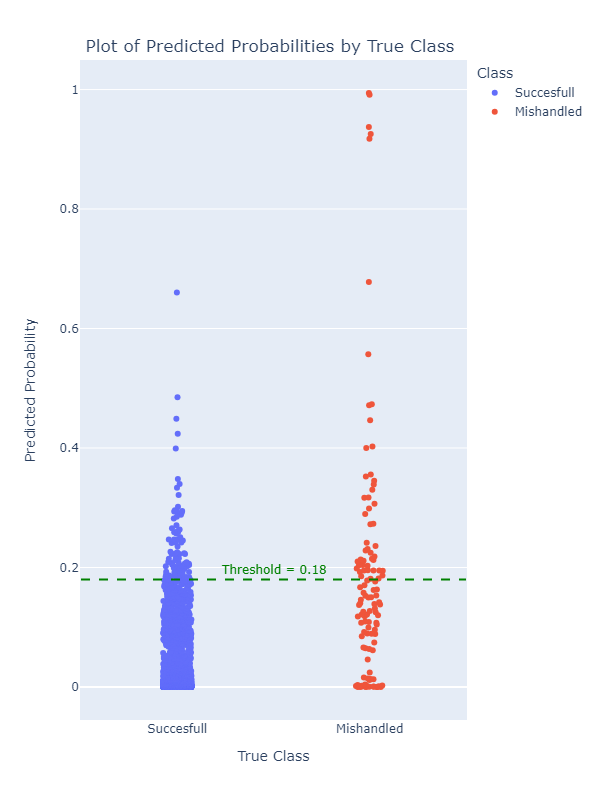
\includegraphics[width=1\textwidth]{Probability_distribution_Model 1.png}\\
    \caption{Predicted score distribution - Logistic regression without path duration}
\end{minipage}
\hfill
\begin{minipage}[c]{0.4\linewidth}
    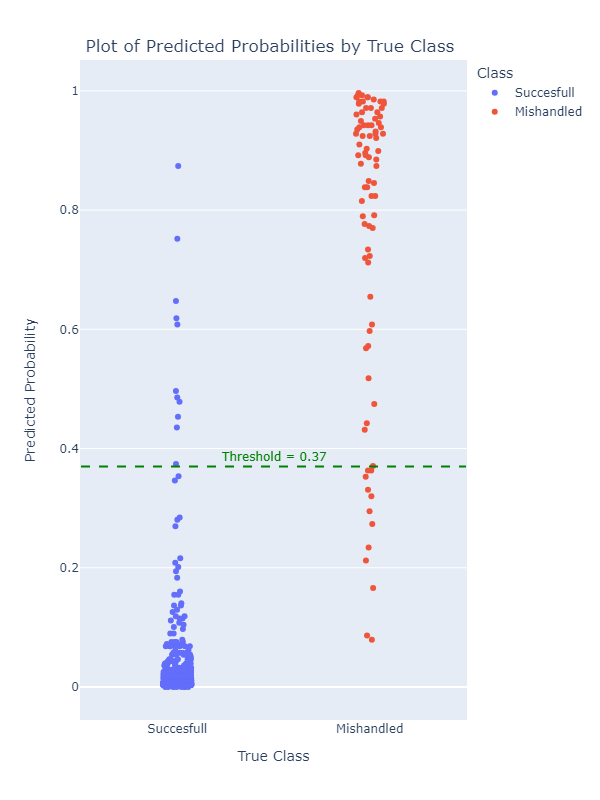
\includegraphics[width=1\textwidth]{Probability_distribution_Model 6.png}\\
    \caption{Predicted score distribution - RF (with path duration)}
\end{minipage}%
\end{figure}
\end{frame}



\begin{frame}{Confusion matrix}
    \begin{figure}
    \begin{minipage}[c]{0.45\linewidth}
    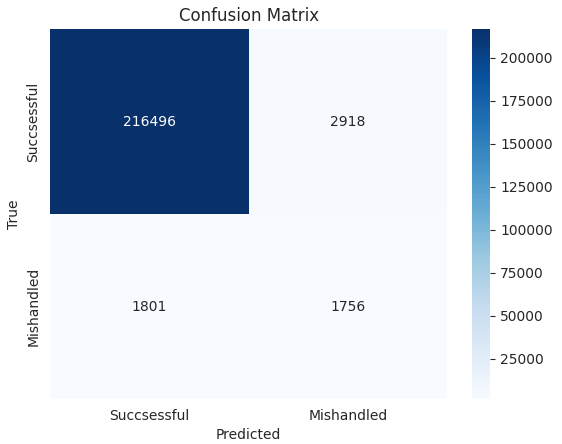
\includegraphics[width=1\textwidth]{Confusion_matrix_Model 1.png}\\
    \caption{Confusion matrix - LR}
\end{minipage}
\hfill
\begin{minipage}[c]{0.45\linewidth}
    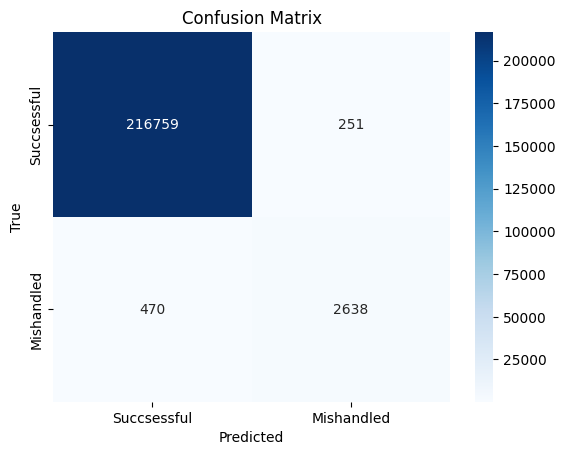
\includegraphics[width=1\textwidth]{Confusion_matrix_Model 6.png}\\
    \caption{Confusion matrix - RF}
\end{minipage}
\end{figure}
\end{frame}


\begin{frame}{Results}
\begin{table}[h]
  \centering
  \caption{Classification results}
  \label{tab:Results}
  \begin{tabular}{|c|c|c|}
        \toprule
        \textbf{Model} & \textbf{F1-Score} & \textbf{AP}  \\
        \midrule
        Logistic regression & 0,43 & 0,39  \\
        Random Forest & 0,88 & 0,93  \\
        XGBoost & 0,89 & 0,93  \\
        \bottomrule
  \end{tabular}
\end{table}
\end{frame}





\begin{frame}{Probability calibration analysis}
\begin{figure}[h]
    \centering
    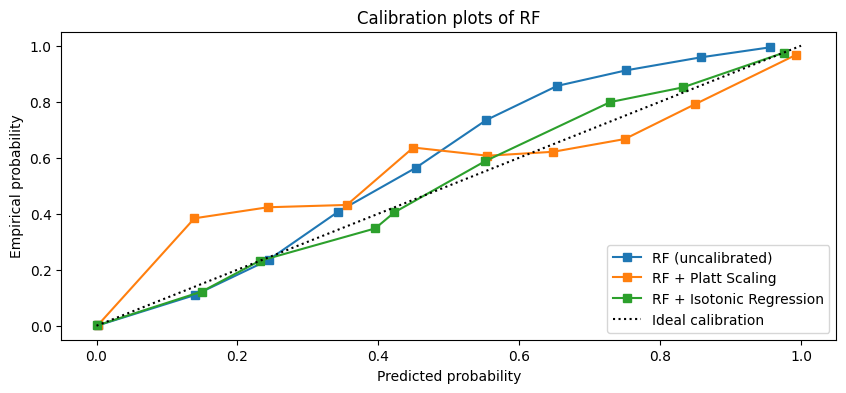
\includegraphics[width=0.8\textwidth]{Calibration_plot_RF.png}\\
    \caption{Probability calibration for RF}
    \label{fig:Probability calibration for rf}
\end{figure}
\end{frame}






\begin{frame}{Conclusion} 
    \begin{itemize}
        \item Results:
            \begin{itemize}
                \item XGBoost and Random Forest are pretty efficient to classify mishandled baggage.
                \item Better F1-Score than in previous studies.
                \item Able to provide probabilities instead of classification.
                \item Path duration have an important impact on the predictions. Using their predicted values can be interesting.
                \item No need to perform under or over-sampling methods.
            \end{itemize}
        \item Limitations:
            \begin{itemize}
                \item Models focused on "feasible" baggage.
                \item Trained and tested for three months only.
            \end{itemize}
        \item Further research suggestions:
            \begin{itemize}
                \item Improving the data quality.
                \item Train for the entire year and include the "month of year" feature.
                \item Test for a date where there was a lot of mishandled baggage.
                \item Find the least important variables (agnostic methods) to drop them and reduce model complexity.
                \item Define the actual cost of a mishandled bag (being injected and rejected), to set up a new optimal classification threshold.
            \end{itemize}
    \end{itemize}
\end{frame}





\begin{frame}{Descriptive statistics} 

\begin{figure}[h]
    \centering
    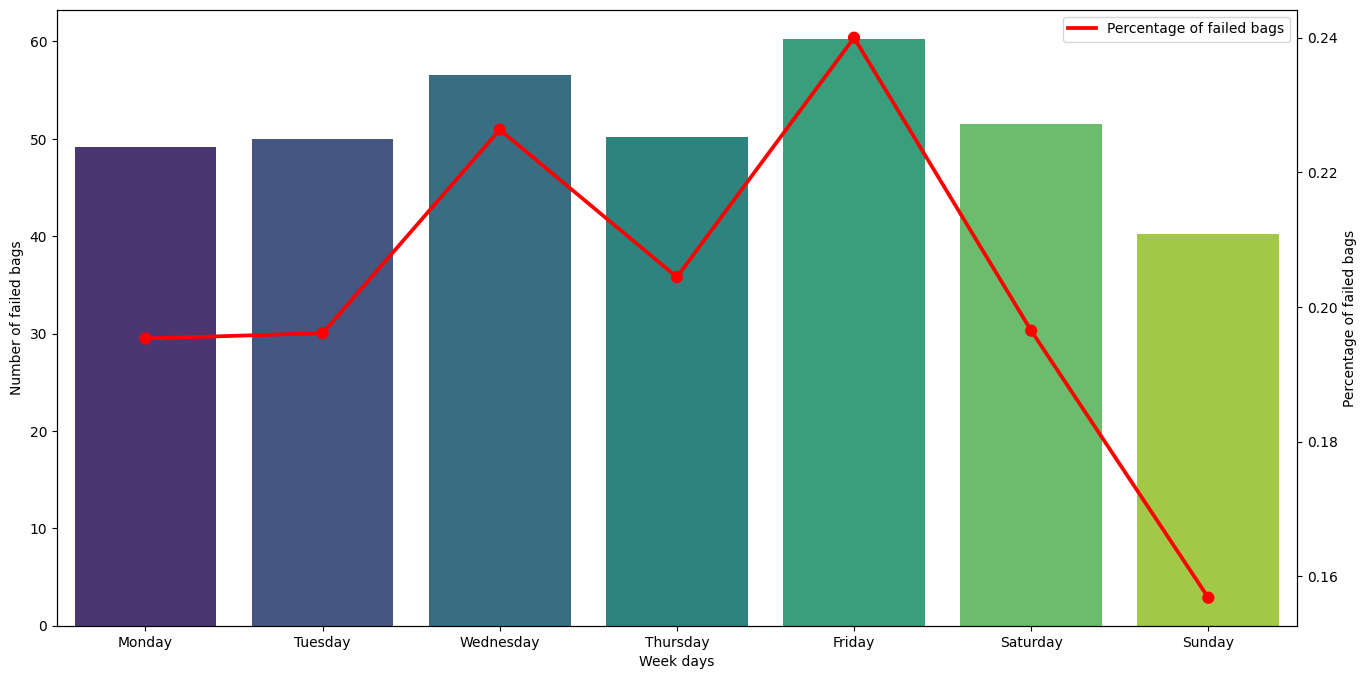
\includegraphics[width=0.9\textwidth]{Number and percentage of failed bags within a week.png}\\
    \caption{Average number and percentage of mishandled bags each days of the week}
    \label{fig:Average number and percentage of mishandled bags each days of the week}
\end{figure}
\end{frame}







\begin{frame}{Descriptive statistics} 
    \begin{figure}[h]
        \centering
        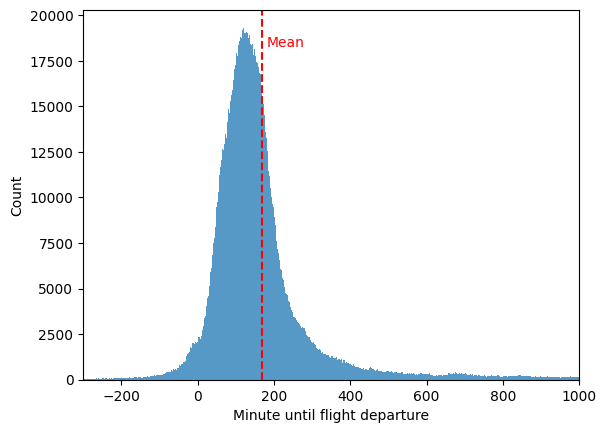
\includegraphics[width=0.6\textwidth]{Minute until flight departure.png}\\
        \caption{Minute until flight departure distribution}
        \label{fig:Minute until flight departure distribution}
    \end{figure}
\end{frame}



\begin{frame}{Descriptive statistics}
    \begin{figure}[ht]
      \centering
      \begin{subfigure}{0.48\textwidth}
        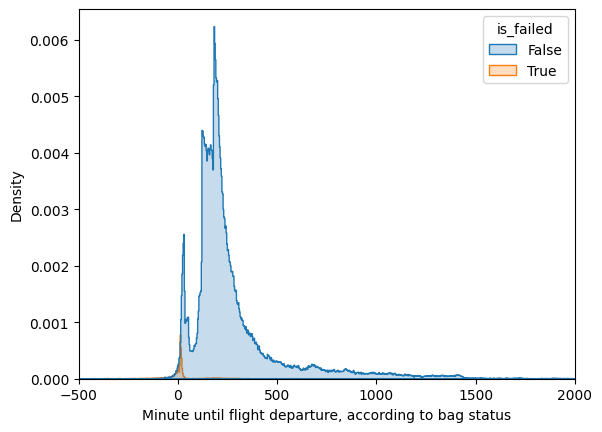
\includegraphics[width=\linewidth]{Minute until flight departure_2.png}
        \caption{Macro view}
      \end{subfigure}
      \hfill
      \begin{subfigure}{0.48\textwidth}
        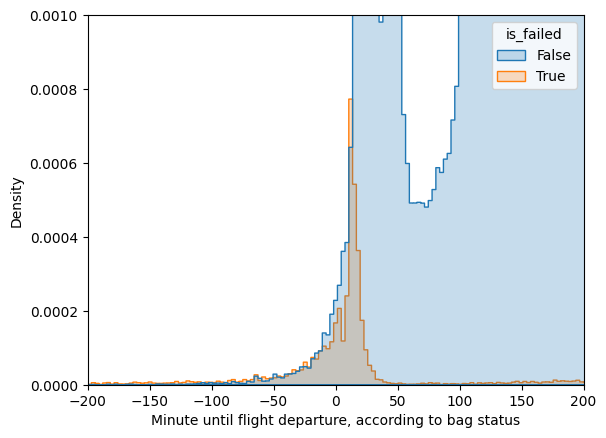
\includegraphics[width=\linewidth]{Minute until flight departure_3.png}
        \caption{Micro view}
      \end{subfigure}
      \caption{Minute until flight departure density according to bag status}
      \label{fig:Minute until flight departure distribution according to bag status}
    \end{figure}
\end{frame}





\end{document}

